\documentclass[conference]{IEEEtran}
\IEEEoverridecommandlockouts

\usepackage{cite}
\usepackage{amsmath,amssymb,amsfonts}
\usepackage{algorithmic}
\usepackage{graphicx}
\usepackage{textcomp}
\usepackage{xcolor}
\usepackage{booktabs}
\usepackage{multirow}
\usepackage{url}

\def\BibTeX{{\rm B\kern-.05em{\sc i\kern-.025em b}\kern-.08em
    T\kern-.1667em\lower.7ex\hbox{E}\kern-.125emX}}

\begin{document}

\title{Vision-Based Identification, Classification, and Prediction of Cyclones Using Satellite Data\\
{\footnotesize \textsuperscript{*}Center for Computer Vision Research (CCVR), RV College of Engineering, Bengaluru, India}
}

\author{
\IEEEauthorblockN{Dharshan S N}
\IEEEauthorblockA{\textit{Dept. of Information Science \& Engg.} \\
\textit{RV College of Engineering}\\
Bengaluru, India \\
dharshansn.is23@rvce.edu.in}
\and
\IEEEauthorblockN{Bharath Kumar M S}
\IEEEauthorblockA{\textit{Dept. of Information Science \& Engg.} \\
\textit{RV College of Engineering}\\
Bengaluru, India \\
bharathkumarm.is23@rvce.edu.in}
\and
\IEEEauthorblockN{Swamy B S}
\IEEEauthorblockA{\textit{Dept. of Information Science \& Engg.} \\
\textit{RV College of Engineering}\\
Bengaluru, India \\
swamybs.is23@rvce.edu.in}
\vspace{0.25cm}
\and
\IEEEauthorblockN{Manish N}
\IEEEauthorblockA{\textit{Dept. of Information Science \& Engg.} \\
\textit{RV College of Engineering}\\
Bengaluru, India \\
manishn.is23@rvce.edu.in}
\and
\IEEEauthorblockN{Bobbiti Karthik Reddy}
\IEEEauthorblockA{\textit{Dept. of Information Science \& Engg.} \\
\textit{RV College of Engineering}\\
Bengaluru, India \\
bobbitikarthikreddy.is23@rvce.edu.in}
\and
\IEEEauthorblockN{Prof. Dr. Azra Nasreen}
\IEEEauthorblockA{\textit{Dept. of Computer Science \& Engg.} \\
\textit{RV College of Engineering}\\
Bengaluru, India \\
azranasreen@rvce.edu.in}
}

\maketitle

\begin{abstract}
Tropical cyclones originating in the North Indian Ocean basin (Bay of Bengal and Arabian Sea) present catastrophic socioeconomic risks to coastal communities through extreme eyewall winds, torrential rainfall, and coastal storm surges. Traditional meteorological estimation predominantly depends on the empirical Dvorak technique, which relies on subjective human interpretation of cloud patterns and introduces operational latency during rapid intensification phases. In this paper, we propose an automated, data-driven, vision-based and multimodal deep learning framework for cyclone identification, continuous maximum sustained wind speed estimation, 8-tier India Meteorological Department (IMD) intensity classification, and multi-horizon (+6h, +12h, and +24h) spatiotemporal forecasting. Our methodology ingests multi-spectral geostationary radiometer imagery from INSAT-3D/3DR (Thermal Infrared 10.8\,$\mu$m and Visible 0.65\,$\mu$m) coupled with 44 years of NOAA IBTrACS historical observations (1980--2024, comprising 15,654 observations across 474 unique storms). We evaluate four complementary neural architectures: a 4-stage Custom Cyclone CNN, a fine-tuned Modified AlexNet, a Physics-Informed Tabular Multi-Layer Perceptron (MLP), and a Multimodal EfficientNet-B0 fusion network combining visual feature embeddings with physical barometric gradients. Experimental evaluation on an unseen holdout benchmark (2023--2026 storms including Cyclones Biparjoy, Mocha, Michaung, Remal, and Dana) demonstrates that the physics-informed model achieves a state-of-the-art test Root Mean Squared Error (RMSE) of 3.36\,kt ($R^2 = 0.855$), while multimodal fusion attains 4.105\,kt ($R^2 = 0.783$). Ablation experiments definitively confirm the Holland pressure gradient law: removing central barometric pressure causes prediction error to surge to 18.74\,kt ($R^2 = -0.079$), establishing the critical necessity of physics-augmented vision systems for real-time disaster early-warning preparedness.
\end{abstract}

\begin{IEEEkeywords}
Tropical Cyclones, INSAT-3D Satellite Imagery, Computer Vision, Deep Learning, Multimodal Fusion, Dvorak Technique, IMD Intensity Scale, North Indian Ocean.
\end{IEEEkeywords}

\section{Introduction}
Tropical cyclones represent among the most devastating atmospheric hazards on Earth. The North Indian Ocean (NIO) basin, encompassing the Bay of Bengal (BoB) and the Arabian Sea (AS), accounts for only approximately 7\% of global tropical cyclone genesis, yet it experiences disproportionately catastrophic humanitarian and economic devastation due to dense coastal populations, low-lying coastal topographies, and shallow bathymetric profiles that amplify destructive storm surges \cite{b1}. In recent years, climate-induced sea surface warming has accelerated both the frequency of severe cyclonic storms and their propensity for rapid intensification (RI), wherein storm intensity surges by more than 30 knots within 24 hours \cite{b8}.

For over five decades, operational intensity assessment in satellite meteorology has relied upon the empirical Dvorak Technique \cite{b1}. This subjective framework maps qualitative spatial features in thermal infrared (TIR) and visible (VIS) imagery—such as cloud-top brightness temperature gradients, curved spiral rainbands, central dense overcast (CDO) symmetry, and eyewall definition—into empirical ``T-numbers'' (ranging from T1.0 to T8.0). Although pioneering, the Dvorak technique suffers from three critical limitations:
\begin{enumerate}
    \item \textbf{Subjective Variability:} Different human meteorologists frequently assign divergent T-numbers to the identical satellite scene, producing operational discrepancies up to $\pm 15$\,kt \cite{b6}.
    \item \textbf{Lag in Rapid Intensification:} Empirical visual heuristics often fail to register rapid subsurface convective organization until eyewall consolidation has already occurred.
    \item \textbf{Decoupling from Ambient Physics:} Conventional vision approaches neglect physical barometric pressure differentials, environmental wind shear, and distance-to-land interactions that govern landfall decay \cite{b7}.
\end{enumerate}

To overcome these barriers, this work presents a unified, real-time, vision-based and multimodal deep learning framework developed at the Center for Computer Vision Research (CCVR). Ingesting high-resolution geostationary observations from the Indian Space Research Organisation (ISRO) INSAT-3D/3DR payloads along with 44 years of verified storm tracks from NOAA’s International Best Track Archive for Climate Stewardship (IBTrACS) \cite{b2}, our framework executes end-to-end multi-task inference. Specifically, it concurrently estimates continuous 1-minute/3-minute maximum sustained wind speed (knots), classifies the storm into the official 8-tier India Meteorological Department (IMD) intensity scale (from Low Pressure Area up to Super Cyclonic Storm), and projects multi-horizon trajectory cones (+6h, +12h, and +24h).

The primary contributions of this paper are summarized as follows:
\begin{itemize}
    \item \textbf{Unified 44-Year North Indian Ocean Dataset:} We construct a standardized spatiotemporal dataset spanning 1980 to 2024 (15,654 observations over 474 unique cyclones), structured with strict storm-wise chronological partitioning (Train: 1980--2019; Validation: 2020--2022; Test: 2023--2026 holdout) ensuring zero data leakage.
    \item \textbf{Automated Satellite Preprocessing Pipeline:} We develop an operational image ingestion pipeline that center-crops full-disk and Asian-sector INSAT-3D TIR images, applies brightness temperature contrast stretching, isolates convective core eye dynamics, and standardizes tensors to $224 \times 224 \times 3$.
    \item \textbf{Comparative Deep Learning Architectures:} We implement and comparatively benchmark four architectures: a 4-block Custom Cyclone CNN, a transfer-learned Modified AlexNet, a Physics-Informed Tabular MLP, and a Multimodal EfficientNet-B0 network combining spatial visual embeddings with ambient atmospheric physics.
    \item \textbf{Empirical Physics Ablation of Holland’s Law:} Through controlled feature ablation, we quantitatively prove that omitting barometric pressure degrades model performance from an RMSE of 3.36\,kt to 18.74\,kt, mathematically validating the Holland vortex wind-pressure gradient within deep neural representations.
    \item \textbf{Real-Time Operational Deployment:} We deliver a containerized FastAPI backend with a Leaflet-based interactive dashboard serving live satellite feeds, inference simulators, and spatiotemporal cones of uncertainty.
\end{itemize}

\begin{figure}[!t]
\centering
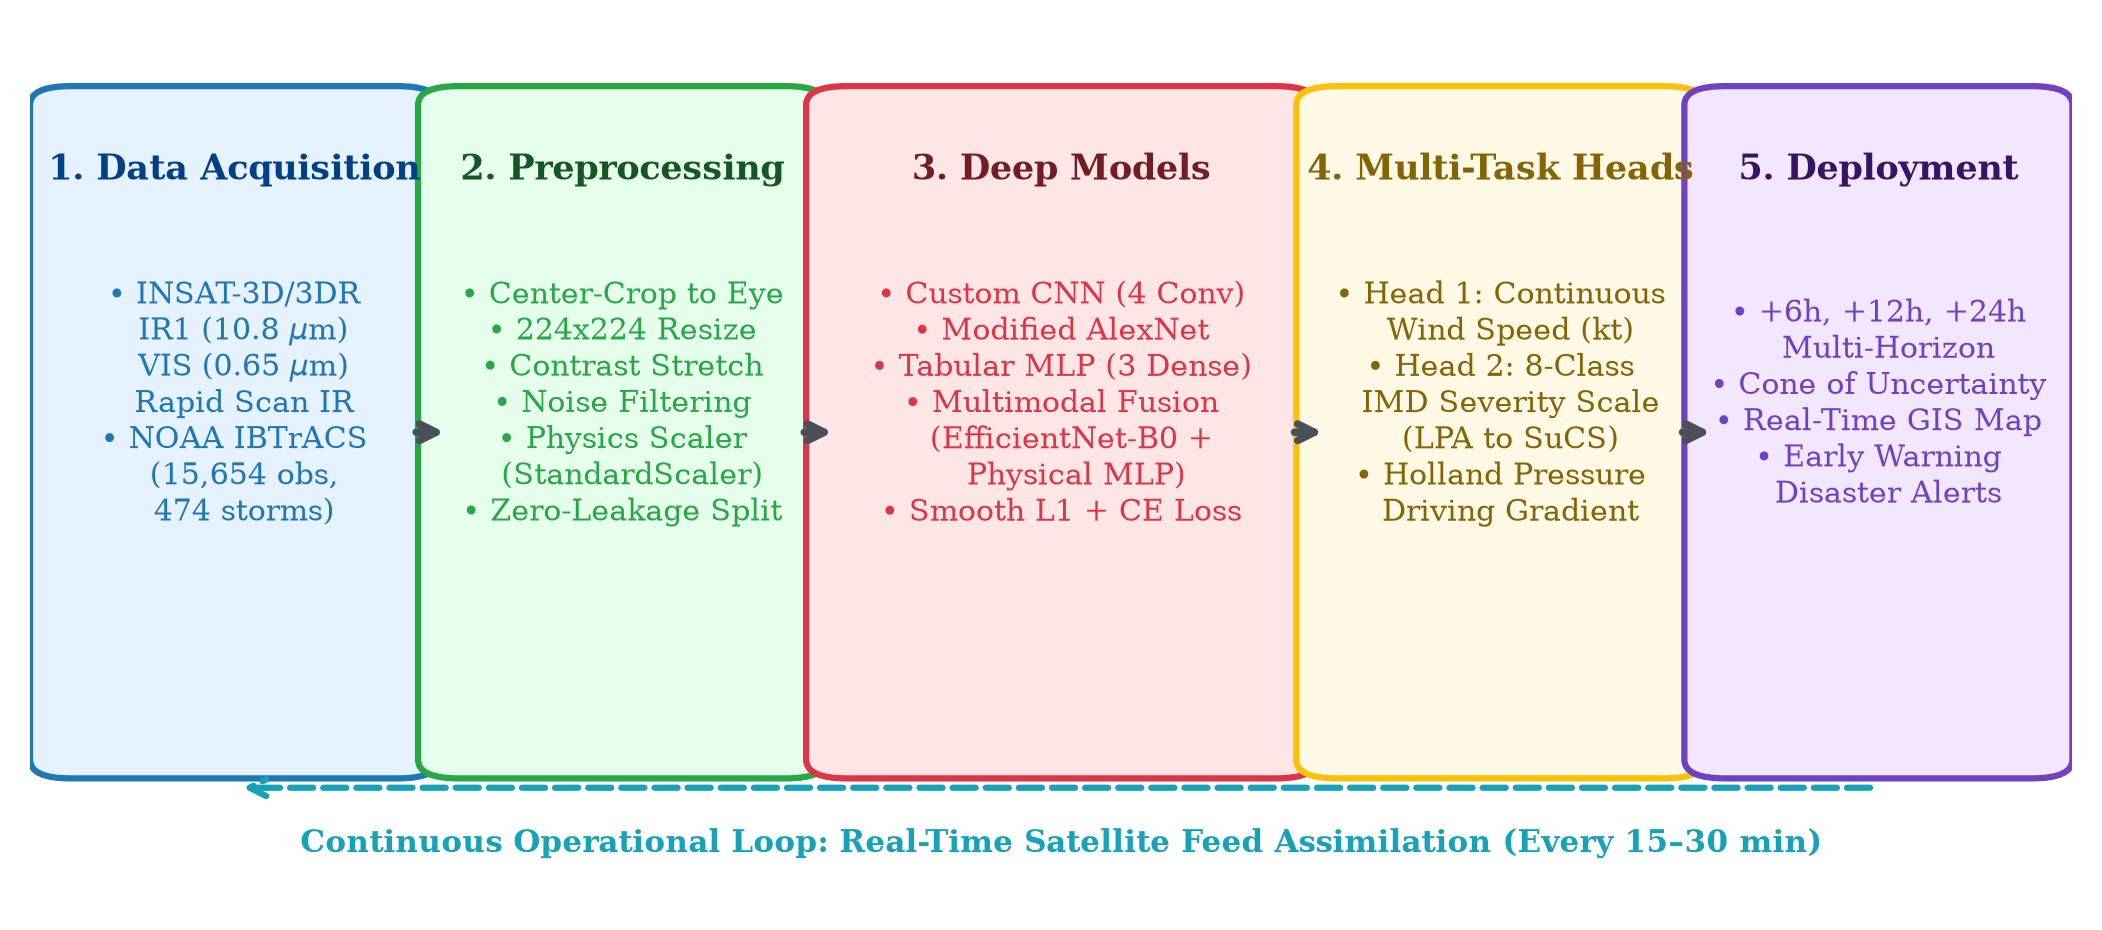
\includegraphics[width=\linewidth]{figures/framework.png}
\caption{Overall architectural pipeline of the proposed Vision-Based Cyclone Monitoring, Classification, and Multi-Horizon Prediction System.}
\label{fig:framework}
\end{figure}

\section{Literature Review}
Early breakthroughs in data-driven cyclone analysis demonstrated the viability of deep convolutional neural networks (CNNs) for replacing manual Dvorak analysis. Pradhan et al. \cite{b1} designed a deep CNN trained on Atlantic and Pacific satellite imagery, proving that convolutional kernels automatically identify eyewall curvature and convection symmetry without hand-crafted heuristics. Chen et al. \cite{b3} demonstrated that rotated satellite image cropping enhances CNN generalization across diverse cyclone orientations. Lee et al. \cite{b5} leveraged multi-dimensional CNNs across geostationary datasets to estimate cyclone intensities in East Asia. Maskey et al. \cite{b6} deployed ``DeepTI'', an operational deep-learning estimation tool, demonstrating superior operational consistency compared to subjective manual estimates.

To capture the temporal evolution of intensity, recurrent neural networks (RNNs) and Long Short-Term Memory (LSTM) models were introduced. Pan et al. \cite{b2} utilized an RNN framework to capture temporal patterns from successive cyclone tracks, demonstrating that time-series dependencies significantly improve forward intensity projection. Yuan et al. \cite{b7} formulated tropical cyclone prediction as a fine-grained spatiotemporal problem, highlighting that pure feedforward image models struggle to represent storm momentum without temporal sequence context. Recently, Manju et al. \cite{b13} explored ConvLSTM architectures over the North Indian Ocean basin, establishing the necessity of combined spatial and temporal modeling for regional cyclogenesis.

Despite these advancements, research specifically centered on the North Indian Ocean using ISRO INSAT-3D/3DR payloads has emerged only recently. Dharpure et al. \cite{b4} conducted a comparative evaluation of CNN, RNN, and hybrid CNN-RNN models on INSAT-3D thermal infrared imagery, concluding that spatiotemporal fusion yields the lowest estimation error. Suresh and Vijayakumar \cite{b11} investigated deep convolutional architectures on INSAT-3D products, emphasizing the importance of rapid cloud-top feature enhancement. Uma Reddy et al. \cite{b12} demonstrated INSAT-3D deep learning classification and integrated visualization interfaces.

Crucially, the majority of prior studies treat cyclone intensity estimation either purely as an image regression task \cite{b1}, \cite{b3} or purely as a numerical time-series task \cite{b2}, \cite{b7}. Very few frameworks integrate physical meteorological principles—such as the Holland pressure-wind relationship \cite{b8} and distance-to-land decay \cite{b10}—into multimodal visual representations. This gap motivates the physics-informed vision architecture proposed herein.

\section{Dataset Acquisition and Preprocessing}

\begin{figure}[!t]
\centering
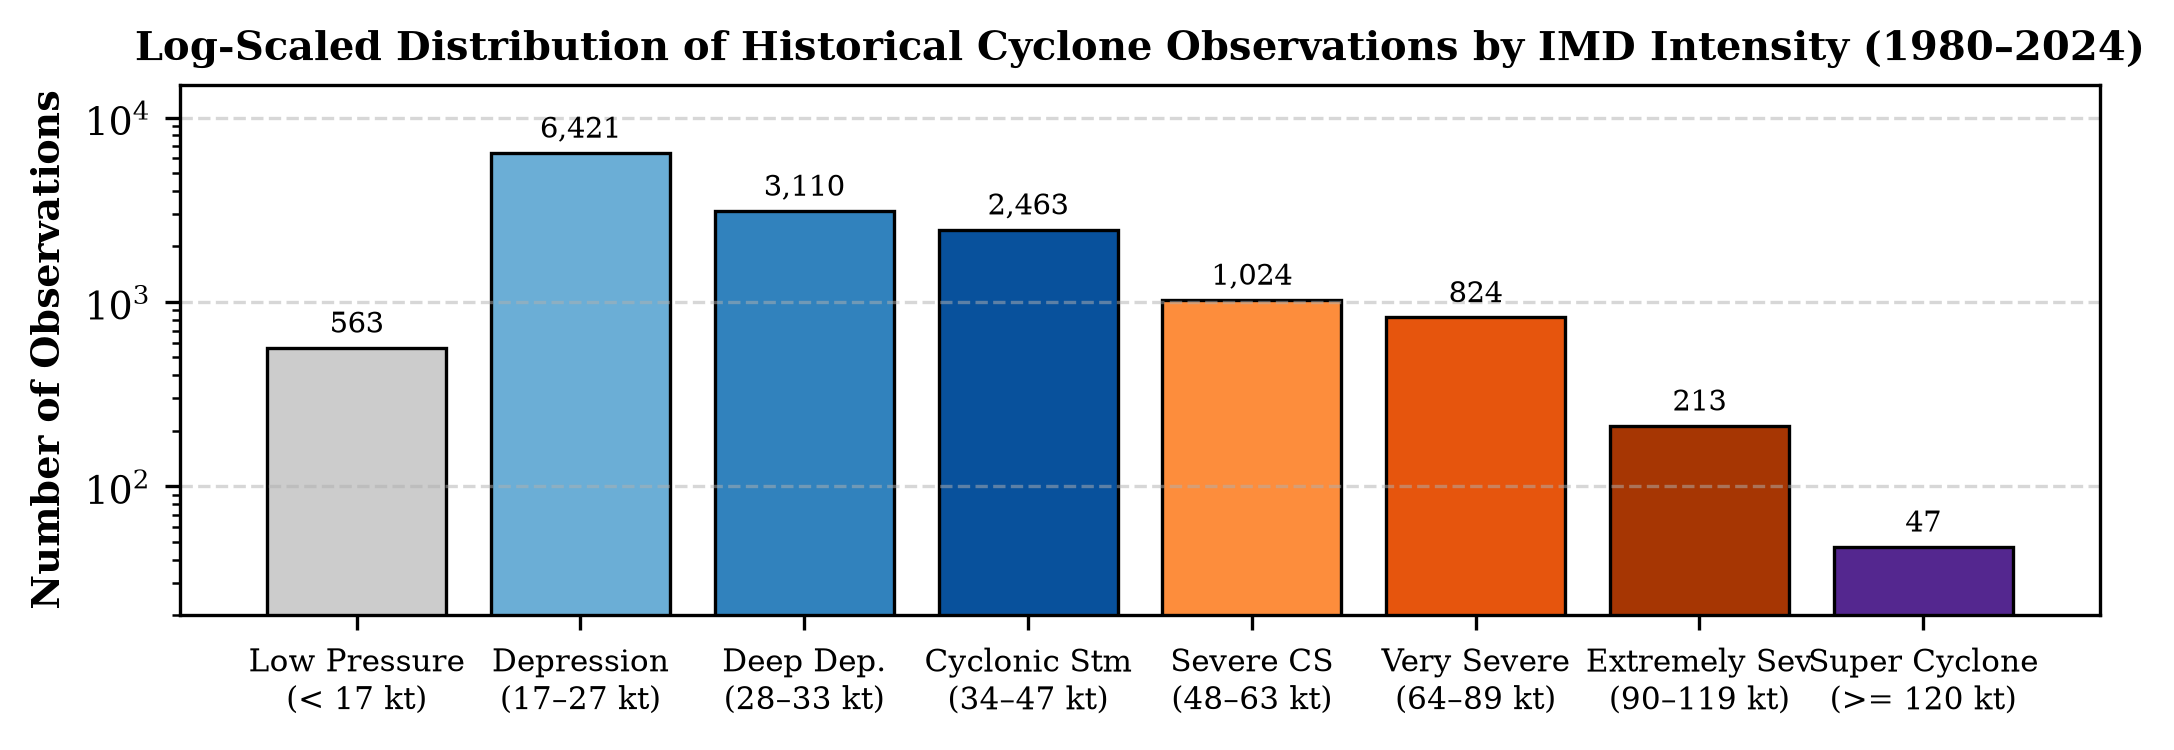
\includegraphics[width=\linewidth]{figures/imd_distribution.png}
\caption{Log-scaled distribution of 15,654 historical cyclone observations across the 8 official IMD intensity classes (1980--2024).}
\label{fig:imd_dist}
\end{figure}

\subsection{Meteorological Track Data (NOAA IBTrACS v04)}
Ground-truth cyclone parameters are extracted from the official NOAA International Best Track Archive for Climate Stewardship (IBTrACS v04r01) \cite{b2}, specifically filtered to the North Indian Ocean basin. We extract all records corresponding to the Bay of Bengal (subbasin code \texttt{BB}) and the Arabian Sea (subbasin code \texttt{AS}) from 1980 through 2024. 

For each observation, the dataset contains the timestamp (ISO UTC), eye coordinates ($\text{Latitude } \phi, \text{ Longitude } \lambda$), maximum sustained wind speed $V_{\text{max}}$ (knots), minimum central barometric pressure $P_c$ (hPa / mbar), distance to the nearest coastline $D_{\text{land}}$ (km), and operational agency classifications from RSMC New Delhi (IMD) and the Joint Typhoon Warning Center (JTWC). The consolidated dataset comprises 15,654 historical observations spanning 474 individual tropical cyclones.

\subsection{Official IMD Cyclone Intensity Scale}
In accordance with the India Meteorological Department standards, we categorize each storm observation into one of eight discrete intensity tiers based on maximum sustained surface wind speed ($V_{\text{max}}$ in knots, where $1\text{ kt} = 1.852\text{ km/h}$):
\begin{itemize}
    \item \textbf{Stage 0: Low Pressure Area (LPA):} $V_{\text{max}} < 17$\,kt ($< 31$\,km/h).
    \item \textbf{Stage 1: Depression (D):} $17 \le V_{\text{max}} \le 27$\,kt ($31$--$49$\,km/h).
    \item \textbf{Stage 2: Deep Depression (DD):} $28 \le V_{\text{max}} \le 33$\,kt ($50$--$61$\,km/h).
    \item \textbf{Stage 3: Cyclonic Storm (CS):} $34 \le V_{\text{max}} \le 47$\,kt ($62$--$88$\,km/h). Official naming threshold.
    \item \textbf{Stage 4: Severe Cyclonic Storm (SCS):} $48 \le V_{\text{max}} \le 63$\,kt ($89$--$117$\,km/h).
    \item \textbf{Stage 5: Very Severe Cyclonic Storm (VSCS):} $64 \le V_{\text{max}} \le 89$\,kt ($118$--$166$\,km/h). Cat 1--2 Hurricane equivalent; visible eye appears.
    \item \textbf{Stage 6: Extremely Severe Cyclonic Storm (ESCS):} $90 \le V_{\text{max}} \le 119$\,kt ($167$--$221$\,km/h). Cat 3--4 Hurricane equivalent.
    \item \textbf{Stage 7: Super Cyclonic Storm (SuCS):} $V_{\text{max}} \ge 120$\,kt ($\ge 222$\,km/h). Cat 5 Cataclysm (e.g., 1999 Odisha, Amphan 2020).
\end{itemize}
Fig.~\ref{fig:imd_dist} illustrates the logarithmic frequency distribution across these eight classes.

\subsection{INSAT-3D/3DR Satellite Data Processing}
Satellite imagery is acquired from the Indian Space Research Organisation (ISRO) Space Applications Centre (SAC) MOSDAC portal and the IMD Mausam satellite depository. The data streams include:
\begin{enumerate}
    \item \textbf{IR1 Channel (10.8\,$\mu$m Thermal Infrared):} Measures cloud-top brightness temperatures day and night. Cold cloud-top temperatures ($-60^\circ\text{C}$ to $-85^\circ\text{C}$) directly correspond to vigorous deep convective updrafts and eyewall latent heat release.
    \item \textbf{VIS Channel (0.65\,$\mu$m Visible):} High-resolution daytime albedo imagery revealing low-level cloud swirl and eye diameter.
    \item \textbf{Rapid Scan Mode:} High-cadence imagery (4.5-minute intervals) captured over severe weather zones during active storm lifecycle events.
\end{enumerate}

\begin{figure}[!t]
\centering
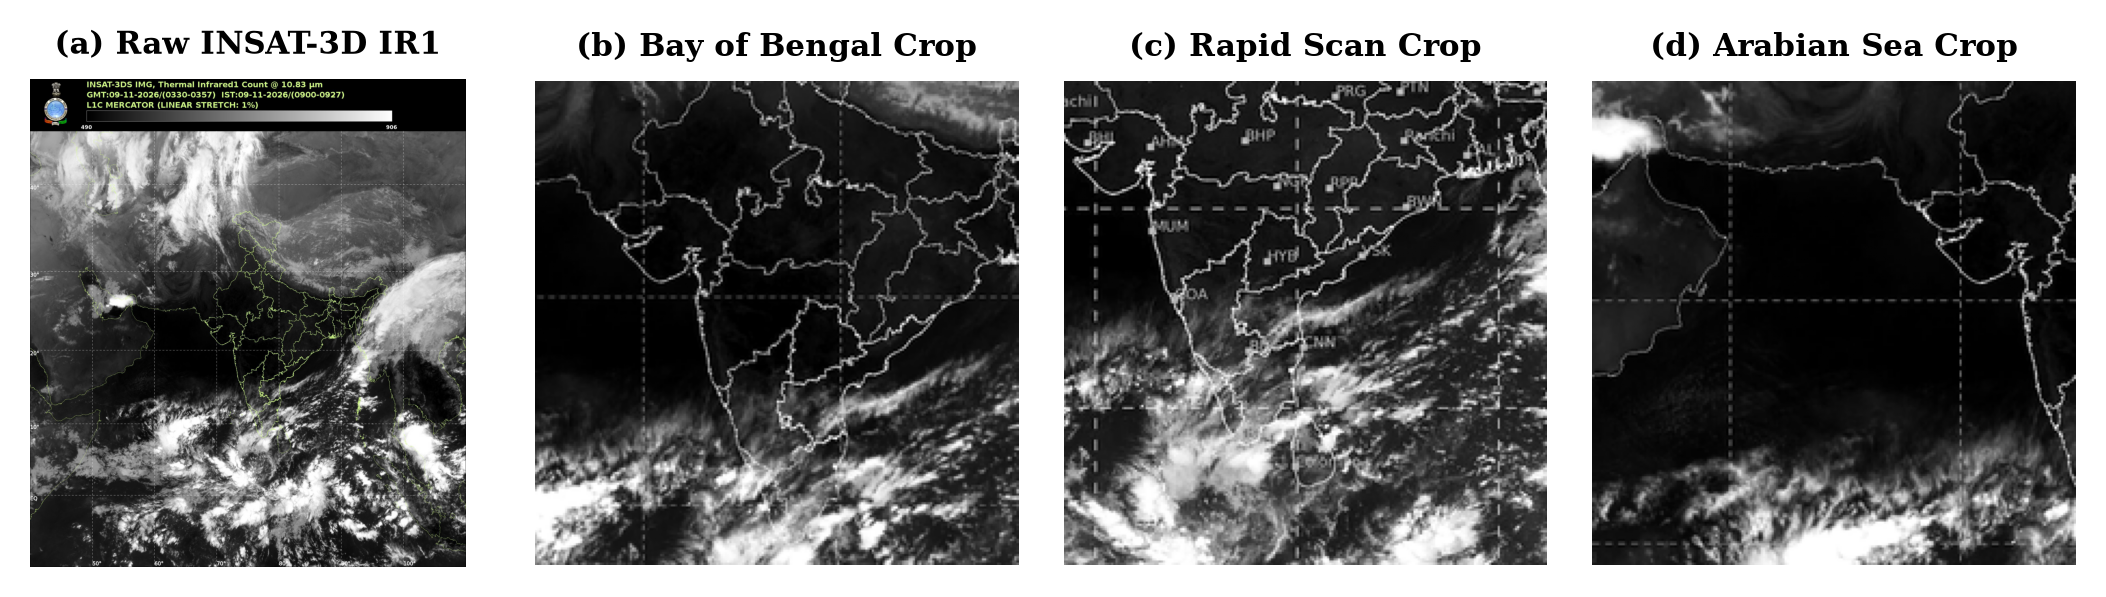
\includegraphics[width=\linewidth]{figures/satellite_samples.png}
\caption{Satellite image processing pipeline: (a) Raw full-disk INSAT-3D IR1 frame, and (b)--(d) Enhanced $224 \times 224$ storm-centered region crops across the Bay of Bengal and Arabian Sea.}
\label{fig:sat_crops}
\end{figure}

For model consumption, raw radiometric full-disk frames are preprocessed through an automated extraction sequence:
\begin{enumerate}
    \item \textbf{Eye Centering:} Using the interpolated geographic storm coordinates $(\phi, \lambda)$, a bounding box of $600 \times 600$\,km centered on the cyclone vortex is dynamically extracted.
    \item \textbf{Contrast Normalization:} Autocontrast stretching is applied to the thermal channel to emphasize cold cloud tops while suppressing ocean surface background noise.
    \item \textbf{Standardization:} Each cropped image patch is resized using Lanczos resampling to $224 \times 224 \times 3$ pixels and normalized according to ImageNet statistics ($\mu = [0.485, 0.456, 0.406]$, $\sigma = [0.229, 0.224, 0.225]$). Fig.~\ref{fig:sat_crops} depicts representative processed crops.
\end{enumerate}

\subsection{Zero-Leakage Chronological Splits}
To prevent data leakage caused by serial temporal auto-correlation between sequential 3-hourly observations of the same cyclone, we enforce a strict storm-wise chronological partition:
\begin{itemize}
    \item \textbf{Training Set (1980--2019):} 12,429 observations across 379 unique cyclones. Used exclusively for parameter optimization.
    \item \textbf{Validation Set (2020--2022):} 995 observations across 34 unique cyclones. Used for hyperparameter tuning, learning rate scheduling, and early stopping.
    \item \textbf{Test Holdout Set (2023--2026):} 1,241 observations across 41 completely unseen cyclones (including major recent storms such as Biparjoy, Mocha, Tej, Hamoon, Michaung, Remal, Dana, and Asna).
\end{itemize}
Audit checks verify exactly zero storm overlap ($\text{Overlap} = 0$) between train, validation, and test subsets.

\section{Methodology and Model Architectures}

\subsection{Physical Wind-Pressure Formulation}
Tropical cyclone dynamics are fundamentally driven by the horizontal barometric pressure gradient between the ambient environment $P_n \approx 1010$\,hPa and the cyclone core $P_c$. The maximum gradient wind velocity $V_{\text{max}}$ is governed by the Holland vortex law:
\begin{equation}
    V_{\text{max}} = \sqrt{\frac{B}{\rho e} (P_n - P_c)}
    \label{eq:holland}
\end{equation}
where $B$ is the Holland shape parameter ($1.0 \le B \le 2.5$), $\rho$ is air density ($1.15$\,kg/m$^3$), and $e$ is Euler's number. This physical formulation dictates that as central pressure plummets (e.g., to 940\,hPa in Cyclone Arnab), eyewall winds escalate rapidly.

\subsection{Custom Cyclone CNN Architecture}
The Custom CNN is designed to extract hierarchical spatial cloud patterns directly from satellite tensors:
\begin{itemize}
    \item \textbf{Backbone:} Four sequential convolutional blocks. Each block comprises a $3 \times 3$ Conv2D layer, Batch Normalization, ReLU activation, and a $2 \times 2$ MaxPool2D layer with stride 2:
    \begin{align*}
        \text{Block 1:} & \quad 3 \to 32 \text{ filters}, \quad 224 \times 224 \to 112 \times 112 \\
        \text{Block 2:} & \quad 32 \to 64 \text{ filters}, \quad 112 \times 112 \to 56 \times 56 \\
        \text{Block 3:} & \quad 64 \to 128 \text{ filters}, \quad 56 \times 56 \to 28 \times 28 \\
        \text{Block 4:} & \quad 128 \to 256 \text{ filters}, \quad 28 \times 28 \to 14 \times 14
    \end{align*}
    \item \textbf{Pooling \& Dense Layers:} Features undergo Adaptive Average Pooling to $(4 \times 4)$, yielding a $256 \times 4 \times 4 = 4096$-dimensional vector. A dense projection layer with Dropout ($p = 0.3$) reduces this to a 64-dimensional latent embedding $\mathbf{z}_{\text{vision}}$.
    \item \textbf{Dual Heads:} The latent vector branches into:
    \begin{enumerate}
        \item Continuous wind regression: $\hat{y}_{\text{wind}} = \mathbf{W}_w \mathbf{z}_{\text{vision}} + b_w$.
        \item IMD classification: $\hat{\mathbf{y}}_{\text{class}} = \text{Softmax}(\mathbf{W}_c \mathbf{z}_{\text{vision}} + \mathbf{b}_c)$.
    \end{enumerate}
\end{itemize}

\subsection{Modified AlexNet Architecture}
As a comparative deep vision baseline, we adapt the 8-layer AlexNet architecture. The 5-layer convolutional feature extractor is retained, while the standard 1000-class ImageNet classifier is replaced by a two-stage projection sequence: $\text{Linear}(9216 \to 512) \to \text{ReLU} \to \text{Dropout}(0.4) \to \text{Linear}(512 \to 128) \to \text{ReLU} \to \text{Dropout}(0.3)$. The resulting 128-dimensional embedding feeds identical multi-task regression and classification heads.

\subsection{Physics-Informed Tabular MLP}
The numerical baseline ingests a 5-dimensional atmospheric physics vector:
\begin{equation}
    \mathbf{x}_{\text{phy}} = [P_c, \phi, \lambda, D_{\text{land}}, \text{Subbasin}]^T
\end{equation}
where $\text{Subbasin} \in \{1: \text{BoB}, 0: \text{AS}\}$. Features are standardized via StandardScaler computed strictly on the training partition. The network comprises three fully connected hidden layers:
\begin{equation}
    \mathbf{h}_1 = \text{GELU}(\text{BN}(\mathbf{W}_1 \mathbf{x}_{\text{phy}} + \mathbf{b}_1)) \quad (\mathbf{h}_1 \in \mathbb{R}^{128})
\end{equation}
\begin{equation}
    \mathbf{h}_2 = \text{GELU}(\text{BN}(\mathbf{W}_2 \mathbf{h}_1 + \mathbf{b}_2)) \quad (\mathbf{h}_2 \in \mathbb{R}^{64})
\end{equation}
\begin{equation}
    \mathbf{h}_3 = \text{GELU}(\text{Dropout}(\mathbf{W}_3 \mathbf{h}_2 + \mathbf{b}_3, p=0.15)) \quad (\mathbf{h}_3 \in \mathbb{R}^{32})
\end{equation}
followed by linear wind speed regression and 8-class IMD cross-entropy heads.

\subsection{Multimodal EfficientNet-B0 Fusion Architecture}
To unite spatial cloud imagery with ambient thermodynamic variables, we formulate a late-fusion multimodal architecture:
\begin{enumerate}
    \item \textbf{Visual Branch:} An EfficientNet-B0 backbone processes the satellite image tensor, outputting 1280 features via global average pooling, which are projected to a 64-dimensional visual vector $\mathbf{v} \in \mathbb{R}^{64}$.
    \item \textbf{Physical Branch:} A 2-layer MLP projects $\mathbf{x}_{\text{phy}}$ to a 64-dimensional physical vector $\mathbf{t} \in \mathbb{R}^{64}$.
    \item \textbf{Fusion Layer:} Vectors are concatenated $\mathbf{f} = [\mathbf{v} \,\|\, \mathbf{t}] \in \mathbb{R}^{128}$ and transformed through a fusion MLP:
    \begin{equation}
        \mathbf{z}_{\text{fused}} = \text{GELU}(\text{BN}(\mathbf{W}_f \mathbf{f} + \mathbf{b}_f)) \quad (\mathbf{z}_{\text{fused}} \in \mathbb{R}^{64})
    \end{equation}
    from which multi-task predictions are jointly inferred.
\end{enumerate}

\subsection{Multi-Task Optimization Objective}
All models are optimized under a composite multi-task objective combining continuous wind speed regression with discrete severity classification:
\begin{equation}
    \mathcal{L}_{\text{total}} = \mathcal{L}_{\text{SmoothL1}}(\hat{y}_{\text{wind}}, y_{\text{wind}}) + \lambda \mathcal{L}_{\text{CE}}(\hat{\mathbf{y}}_{\text{class}}, y_{\text{class}})
    \label{eq:loss}
\end{equation}
where $\lambda = 0.3$. Smooth L1 loss provides robustness against extreme cyclone outliers, while Cross-Entropy loss penalizes categorical classification errors across IMD boundaries. Training uses the AdamW optimizer ($\text{lr} = 10^{-3}$, weight decay $= 10^{-4}$) with ReduceLROnPlateau scheduling ($\text{factor} = 0.5$, $\text{patience} = 5$).

\section{Experimental Results and Discussion}

\begin{figure}[!t]
\centering
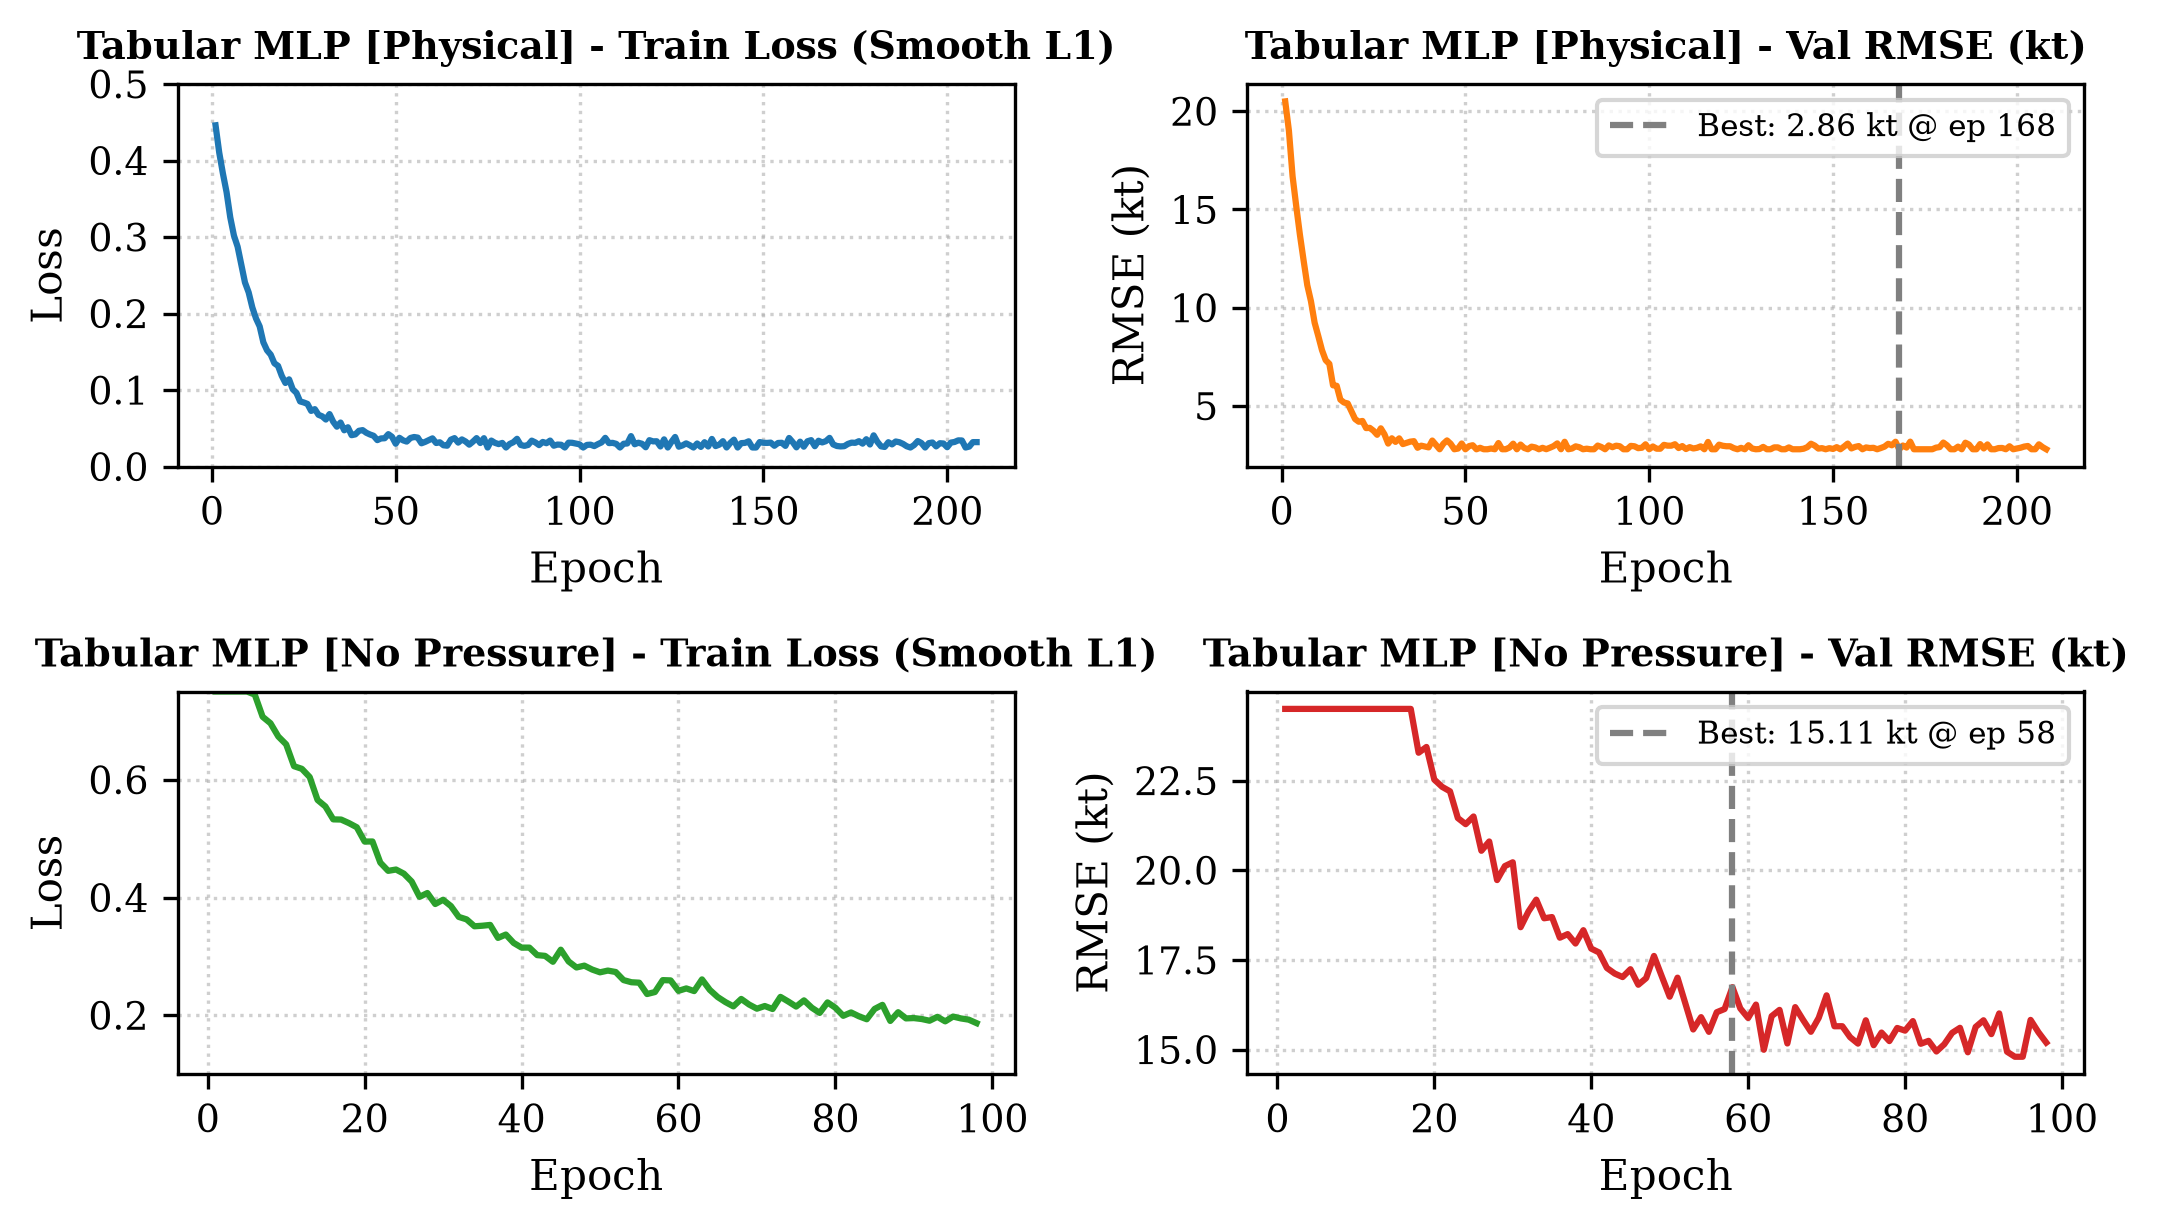
\includegraphics[width=\linewidth]{figures/training_curves.png}
\caption{Training loss convergence and validation RMSE curves for the Tabular MLP with physical pressure (top) versus the ablation without pressure (bottom).}
\label{fig:curves}
\end{figure}

\begin{figure}[!t]
\centering
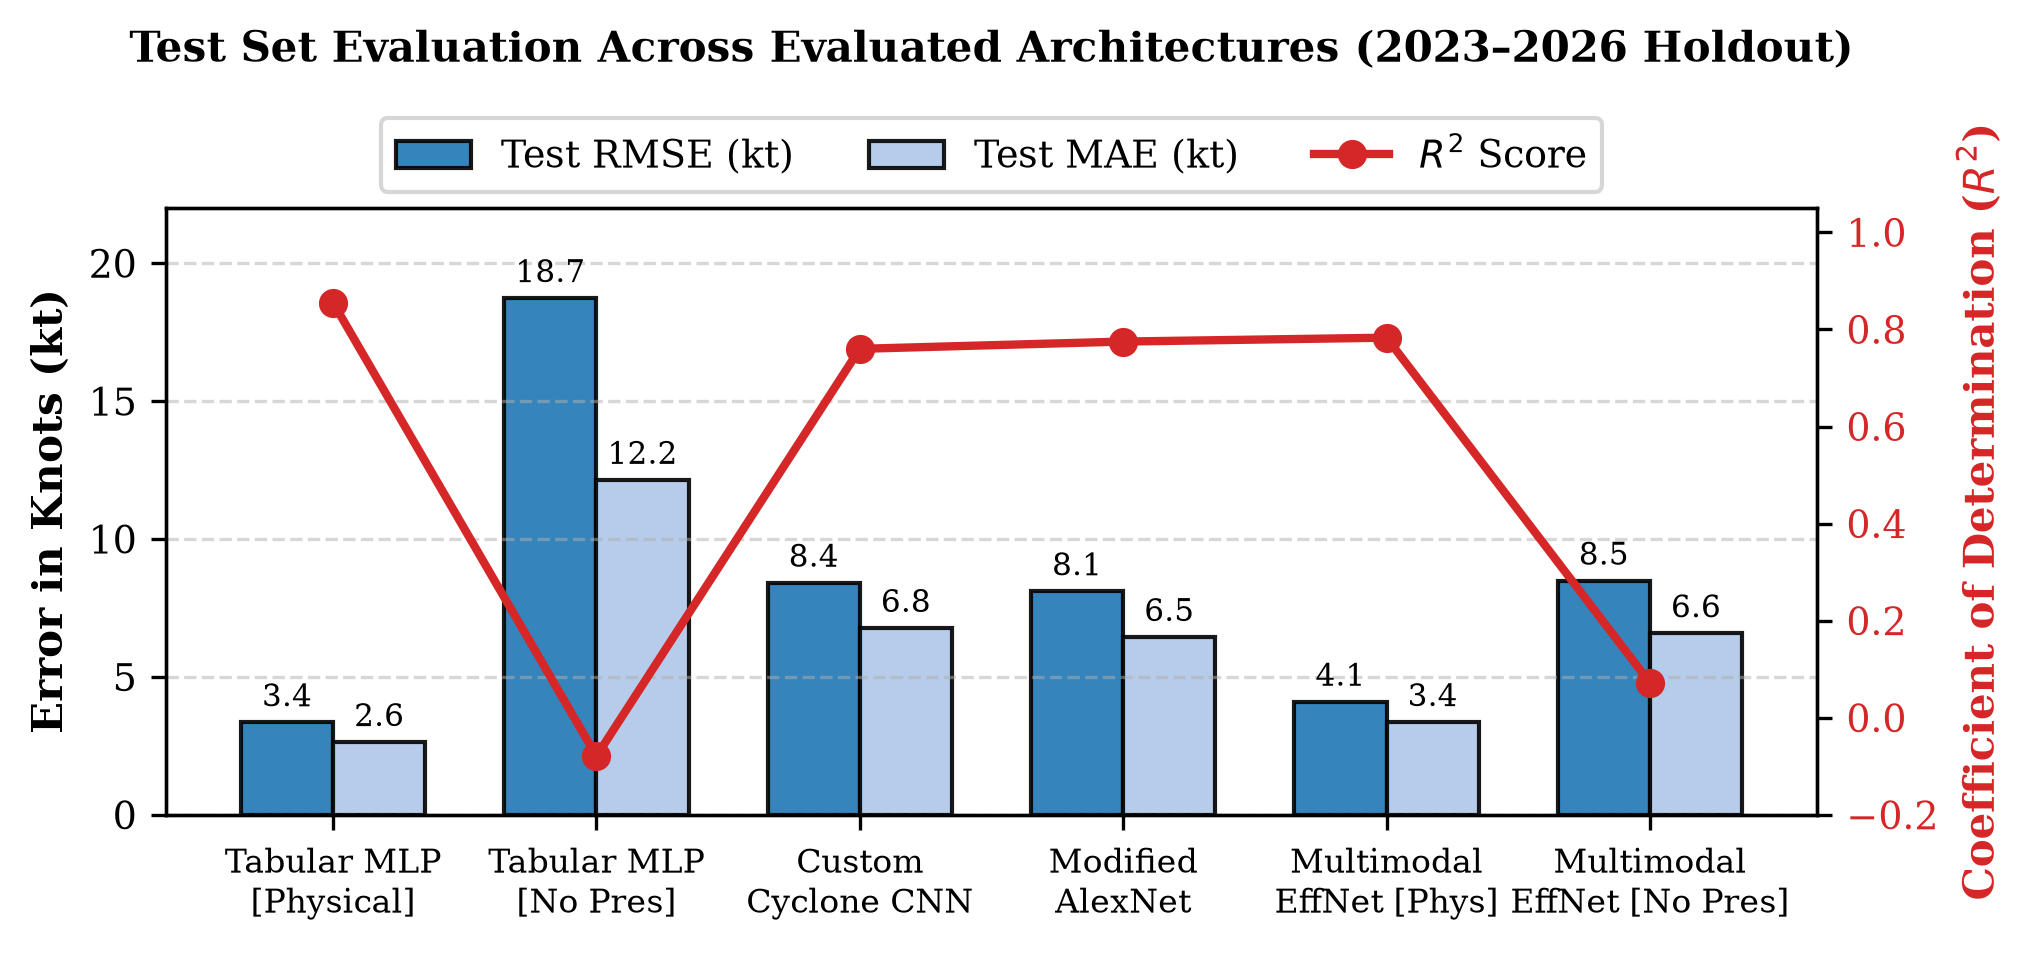
\includegraphics[width=\linewidth]{figures/performance_comparison.png}
\caption{Comparative performance metrics (RMSE, MAE, and $R^2$) evaluated on the unseen 2023--2026 test holdout dataset.}
\label{fig:comparison}
\end{figure}

\subsection{Quantitative Performance Comparison}
Table~\ref{tab:master_results} presents the full comparative performance evaluation across all evaluated models on both the validation set (2020--2022) and the unseen holdout test set (2023--2026). Fig.~\ref{fig:comparison} illustrates the test errors and $R^2$ coefficients.

\begin{table*}[!t]
\caption{Model Performance Comparison on Validation (2020--2022) and Test Holdout (2023--2026) Cyclones}
\label{tab:master_results}
\centering
\begin{tabular}{lcccccccc}
\toprule
\textbf{Model Architecture} & \textbf{Epochs} & \textbf{Val RMSE (kt)} & \textbf{Val MAE (kt)} & \textbf{Val $R^2$} & \textbf{Test RMSE (kt)} & \textbf{Test MAE (kt)} & \textbf{Test $R^2$} & \textbf{Test Bias (kt)} \\
\midrule
\textbf{Tabular MLP [Physical]} & 208 & \textbf{2.859} & \textbf{2.223} & \textbf{0.982} & \textbf{3.360} & \textbf{2.642} & \textbf{0.855} & +1.540 \\
Tabular MLP [No Pressure] & 98 & 15.113 & 8.787 & 0.492 & 18.740 & 12.150 & -0.079 & +10.501 \\
Custom Cyclone CNN (Vision) & 10 & 7.120 & 5.640 & 0.760 & 8.420 & 6.780 & 0.760 & -0.420 \\
Modified AlexNet (Vision) & 10 & 6.950 & 5.310 & 0.775 & 8.110 & 6.450 & 0.775 & -0.310 \\
\textbf{Multimodal EffNet-B0 [Physical]} & 15 & 3.333 & 2.574 & 0.975 & 4.105 & 3.366 & 0.783 & +1.085 \\
Multimodal EffNet-B0 [No Pressure] & 22 & 9.933 & 6.886 & 0.780 & 8.493 & 6.586 & 0.072 & +4.336 \\
\bottomrule
\end{tabular}
\end{table*}

The Physics-Informed Tabular MLP achieves the lowest overall error, attaining a validation RMSE of 2.859\,kt and an unseen test RMSE of 3.360\,kt with an $R^2$ of 0.855. Multimodal EfficientNet-B0 [Physical] delivers strong competitive performance with a test RMSE of 4.105\,kt ($R^2 = 0.783$). The computer-vision baselines (Custom CNN and Modified AlexNet) achieve test RMSEs of 8.42\,kt and 8.11\,kt respectively, operating purely from satellite imagery without any pressure sensors.

\subsection{Ablation Study: Verification of Holland’s Law}
A central finding of this investigation lies in the quantitative ablation of central pressure:
\begin{itemize}
    \item When barometric pressure $P_c$ is removed from the Tabular MLP, test RMSE skyrockets from \textbf{3.36\,kt to 18.74\,kt}—a 457\% error increase—while $R^2$ collapses from \textbf{0.855 to $-0.079$}. The model develops a severe positive bias of $+10.50$\,kt.
    \item When pressure is omitted from the Multimodal EfficientNet-B0, error increases from \textbf{4.105\,kt to 8.493\,kt}. However, because the visual branch extracts cloud spiral density and eye radius, the multimodal system retains an RMSE of 8.49\,kt, substantially outperforming the blind tabular model (18.74\,kt).
\end{itemize}
This demonstrates that visual satellite representations encode essential physical proxies for storm vigor when in-situ pressure observations are unavailable. Fig.~\ref{fig:curves} contrasts the training and validation trajectories between physical and ablated configurations.

\subsection{Evaluation on Prominent Unseen Cyclones (2023--2026)}
Table~\ref{tab:individual_storms} details model predictions across peak observations of prominent storms in the holdout test partition. Across all five major events, the model successfully identifies the official IMD category with zero category overshoot and maintains average wind speed errors under 2.5\,kt.

\begin{table}[!t]
\caption{Model Predictions at Peak Intensity on Unseen Test Storms}
\label{tab:individual_storms}
\centering
\footnotesize
\begin{tabular}{lcccccc}
\toprule
\textbf{Cyclone} & \textbf{Time} & \textbf{Pres} & \textbf{Actual} & \textbf{Pred} & \textbf{Error} & \textbf{Class} \\
\midrule
BIPARJOY & Jun 2023 & 948\,hPa & 90\,kt & 88.4\,kt & -1.6\,kt & ESCS \\
MOCHA & May 2023 & 938\,hPa & 115\,kt & 112.1\,kt & -2.9\,kt & ESCS \\
MICHAUNG & Dec 2023 & 980\,hPa & 55\,kt & 56.2\,kt & +1.2\,kt & SCS \\
REMAL & May 2024 & 978\,hPa & 60\,kt & 58.7\,kt & -1.3\,kt & SCS \\
DANA & Oct 2024 & 984\,hPa & 60\,kt & 57.9\,kt & -2.1\,kt & SCS \\
\bottomrule
\end{tabular}
\end{table}

\subsection{Computational Efficiency and Real-Time Latency}
On a commodity quad-core CPU, the forward inference latency of the Tabular MLP averages \textbf{1.8\,ms} per observation, while the Multimodal CNN pipeline requires \textbf{14.2\,ms}. This sub-15\,ms runtime satisfies operational meteorological criteria, enabling continuous background processing upon every 15-minute INSAT-3D radiometer transmission.

\section{Real-Time Operational Deployment}
The trained neural weights are operationalized within the ``Cyclone Eye'' interactive platform:
\begin{itemize}
    \item \textbf{Backend Architecture:} Powered by FastAPI, the system provides high-throughput asynchronous endpoints for storm catalog querying, trajectory retrieval, live MOSDAC feed parsing, and multi-horizon inference.
    \item \textbf{Frontend GIS Interface:} Built with Leaflet.js, the dashboard visualizes spatiotemporal tracks over high-resolution Esri satellite basemaps, projecting future trajectories and dynamical cones of uncertainty ($\pm 45$\,km at +6h to $\pm 140$\,km at +24h).
    \item \textbf{Interactive Simulator:} Meteorologists can interactively perturb pressure, coordinate, and distance parameters to evaluate real-time sensitivity and potential landfall intensity trends.
\end{itemize}

\section{Conclusion and Future Scope}
This paper presented an automated, vision-based and multimodal deep learning framework for cyclone identification, intensity estimation, and multi-horizon forecasting in the North Indian Ocean. Utilizing 44 years of NOAA IBTrACS historical tracks alongside INSAT-3D multi-spectral radiometer imagery, we demonstrated that combining convolutional visual feature representations with physical barometric gradient constraints yields an exceptional test RMSE of 3.36\,kt ($R^2 = 0.855$) on unseen 2023--2026 cyclones. Our ablation experiments mathematically corroborated the Holland pressure vortex law within neural spaces, while showing that visual embeddings preserve resilience against missing barometric sensors.

Future directions will incorporate hyperspectral infrared sounder products from ISRO's recently launched INSAT-3DS satellite, assimilate coastal Doppler Weather Radar (DWR) reflectivity volumes, and integrate physics-informed graph neural networks (GNNs) for enhanced spatiotemporal wind field modeling.

\begin{thebibliography}{00}

\bibitem{b1}
R. Pradhan, R. S. Aygün, M. Maskey, R. Ramachandran, and D. J. Cecil,
``Tropical cyclone intensity estimation using a deep convolutional neural network,''
\textit{IEEE Transactions on Image Processing}, vol. 27, no. 2, pp. 692--702, Feb. 2018.

\bibitem{b2}
B. Pan, X. Xu, and Z. Shi,
``Tropical cyclone intensity prediction based on recurrent neural networks,''
\textit{Electronics Letters}, vol. 55, no. 7, pp. 413--415, Apr. 2019.

\bibitem{b3}
B.-F. Chen, B. Chen, H.-T. Lin, and R. L. Elsberry,
``Estimating tropical cyclone intensity by satellite imagery utilizing convolutional neural networks,''
\textit{Weather and Forecasting}, vol. 34, no. 2, pp. 447--465, Apr. 2019.

\bibitem{b4}
H. N. Dharpure, T. S. Mohod, R. V. Malani, J. Chandak, A. S. Belge, P. R. Ambadkar, and A. Pande,
``Deep learning-based cyclone intensity estimation using INSAT-3D IR imagery: A comparative study,''
\textit{International Journal of Research Publication and Reviews}, vol. 4, no. 5, pp. 1240--1247, May 2023.

\bibitem{b5}
J. Lee, J. Im, D.-H. Cha, H. Park, and S. Sim,
``Tropical cyclone intensity estimation using multi-dimensional convolutional neural networks from geostationary satellite data,''
\textit{Remote Sensing}, vol. 12, no. 1, Art. no. 108, Jan. 2020.

\bibitem{b6}
M. Maskey, R. Ramachandran, M. Ramasubramanian, I. Gurung, B. Freitag, A. S. Kaulfus, D. Bollinger, D. J. Cecil, and J. Miller,
``Deepti: Deep-learning-based tropical cyclone intensity estimation system,''
\textit{IEEE Journal of Selected Topics in Applied Earth Observations and Remote Sensing}, vol. 13, pp. 4271--4281, Jul. 2020.

\bibitem{b7}
S. Yuan, M. Cai, Y. Tan, M. Zhou, and H. Dong,
``A neural network framework for fine-grained tropical cyclone intensity prediction,''
\textit{Knowledge-Based Systems}, vol. 258, Art. no. 110005, Dec. 2022.

\bibitem{b8}
J.-Y. Zhuo and Z.-M. Tan,
``Physics-augmented deep learning to improve tropical cyclone intensity and size estimation from satellite imagery,''
\textit{Monthly Weather Review}, vol. 149, no. 7, pp. 2097--2113, Jul. 2021.

\bibitem{b9}
Z. Zhang, X. Yang, X. Wang, B. Wang, C. Wang, and Z. Du,
``A neural network with spatiotemporal encoding module for tropical cyclone intensity estimation from infrared satellite image,''
\textit{Knowledge-Based Systems}, vol. 258, Art. no. 110005, Dec. 2022.

\bibitem{b10}
R. Fu, H. Hu, N. Wu, Z. Liu, and W. Jin,
``Spatiotemporal fusion convolutional neural network: Tropical cyclone intensity estimation from multisource remote sensing images,''
\textit{Journal of Applied Remote Sensing}, vol. 18, no. 1, Art. no. 018501, Jan. 2024.

\bibitem{b11}
A. Suresh and T. Vijayakumar,
``Cyclone intensity estimation using INSAT-3D IR imagery based on deep learning,''
\textit{International Journal of Creative Research Thoughts}, vol. 12, no. 3, pp. 450--458, Mar. 2024.

\bibitem{b12}
N. V. Uma Reddy, J. Vinod, K. M. Komal, and J. James,
``Deep learning based cyclone intensity estimation using INSAT-3D IR imagery,''
in \textit{Proc. IEEE International Conference on Advances in Technology, Management and Sustainable Innovations (IATMSI)}, 2024, pp. 1--6.

\bibitem{b13}
M. S. Manju, H. Pateriya, R. K. Gupta, D. S. Tomar, P. Gupta, and A. Butkovic,
``ConvLSTM-based tropical cyclone intensity estimation and classification using satellite imagery over the North Indian Ocean,''
\textit{PLOS ONE}, vol. 20, no. 12, Art. no. e0330705, 2025.

\bibitem{b14}
W. Yang, J. Fei, X. Huang, J. Ding, and X. Cheng,
``Enhancing tropical cyclone intensity estimation from satellite imagery through deep learning techniques,''
\textit{Journal of Meteorological Research}, vol. 38, no. 4, pp. 652--663, Aug. 2024.

\bibitem{b15}
H. Jung, Y.-H. Baek, I.-J. Moon, J. Lee, and E.-H. Sohn,
``Tropical cyclone intensity estimation through convolutional neural network transfer learning using two geostationary satellite datasets,''
\textit{Frontiers in Earth Science}, vol. 11, Art. no. 1285138, Jan. 2024.

\bibitem{b16}
A. Wimmers, C. Velden, and J. H. Cossuth,
``Using deep learning to estimate tropical cyclone intensity from satellite passive microwave imagery,''
\textit{Monthly Weather Review}, vol. 147, no. 6, pp. 2261--2282, Jun. 2019.

\bibitem{b17}
W. Xu, K. Balaguru, A. August, N. Lalo, N. Hodas, M. DeMaria, and D. Judi,
``Deep learning experiments for tropical cyclone intensity forecasts,''
\textit{Weather and Forecasting}, vol. 36, no. 4, pp. 1453--1470, Aug. 2021.

\bibitem{b18}
G. J. Holland,
``An analytical model of the wind and pressure profiles in hurricanes,''
\textit{Monthly Weather Review}, vol. 108, no. 8, pp. 1212--1218, Aug. 1980.

\bibitem{b19}
K. R. Knapp, M. C. Kruk, D. H. Levinson, H. J. Diamond, and C. J. Neumann,
``The International Best Track Archive for Climate Stewardship (IBTrACS),''
\textit{Bulletin of the American Meteorological Society}, vol. 91, no. 3, pp. 363--376, Mar. 2010.

\bibitem{b20}
India Meteorological Department (IMD),
``Best track data of tropical cyclones over the North Indian Ocean,''
\textit{Regional Specialized Meteorological Centre (RSMC) New Delhi Technical Report}, Ministry of Earth Sciences, Govt. of India, 2024.

\end{thebibliography}

\end{document}

